\section{Detection Mechanism and Interface Prototyping}
\subsection{Harpishcord Register Staggering}
\subsection{Force Sensing Resistors}
\subsection{Measurement of Pressure Data}
\section{Interacting with Real-Time Audio Software}


\section{Introduction} 
\label{sec:introduction}
The evolution of digital sound synthesis has transformed the relationship between human gesture, performance, and sound production. Early digital instruments offered sonic flexibility but introduced a degree of abstraction, primarily due to reliance on indirect parameter manipulation rather than direct physical interaction \cite{roads1996computer, moore1990elements}. With advances in computational power, real-time processing and expressive controllers have reintroduced immediacy to digital performance, allowing musicians to interact with sound more intuitively \cite{trolland2022airsticks,caren2020keywi,mcpherson2013space}. Nevertheless, the fundamental challenge of expressive control remains central across domains such as live electronic music and interactive performance systems, where continued exploration has led to the creation of complex multimodal interfaces \cite{tanaka2002multimodal}.

The challenge of control remains open and becomes relevant when applied to historical musical instruments, where physical fragility often precludes direct interaction \cite{mcalpine2014sampling,baldwin2016tromba,nemus2025erc}. Physical modelling synthesis presents a promising solution by enabling real-time simulation of an instrument’s behaviour \cite{smith2010physical, bilbao2009numerical}. However, digital reconstructions often struggle to capture the fine-grained control and responsiveness required for historically informed performance practices.

The harpsichord exemplifies this difficulty. Characterised by its distinctive articulation and multiple registers, it requires nuanced control to produce its characteristic sound \cite{kottick1991acoustics}. In traditional harpsichords, jack staggering creates intentional time offsets between multiple plucks triggered by the same key \cite{diveroli2012harpsichord}. This prevents the player from engaging multiple strings with excessive force simultaneously. Yet, such subtle timing is often overlooked in sample-based libraries, where a single MIDI note triggers all registers simultaneously. Standard MIDI keyboards compound the issue, lacking the tactile feedback and mechanical complexity necessary to replicate historical instruments’ expressive intricacies—especially the delayed plucks across registers. Previous work has enhanced a museum-based keyboard replica with a sensor system \cite{hamilton2025augmentation} to control a commercial sample library, but sample-based implementations remain fundamentally limited. The core issue lies in their one-to-one mapping of MIDI events to sound triggers.

This paper introduces a novel control interface designed to overcome these constraints. By incorporating a custom sensing system that independently tracks the movement of each register, the proposed design enables precise articulation and timing control. This restores essential performance characteristics of historical harpsichords and strengthens the link between digital synthesis and authentic historical expression. 
A public repository containing supplementary material is available\footnote{\href{https://github.com/Nemus-Project/modal-harpsichord}{https://github.com/Nemus-Project/modal-harpsichord}}. In particular, videos demonstrating the pluck detection mechanism are relevant for supporting the results discussed in the following section. 

\section{Detection Mechanism and Interface Prototyping}

Rather than relying on commercial weighted-key MIDI controllers—which fail to replicate the mechanical resistance profile of a harpsichord~\cite{mcalpine2014sampling}—a physical prototype of the harpsichord mechanism was commissioned from a professional instrument maker. The prototype includes three keys, each coupled to two jacks tuned in unison (Figure~\ref{fig:3-key-model}). While scaled down and unpitched, the string selection and mechanical dimensions were informed by a luthier to approximate the C2–D2 register with comparable tension and gauge. Each key acts as a class-1 lever, lifting jacks from different points along its length. This staggered design results in varying jack velocities, influencing the timing of plucks. 
\begin{figure}
    \centering
    \includegraphics[width=1\linewidth]{img/model-top-2.png}\\
    \includegraphics[width=1\linewidth]{img/3-key-side.png}
    \caption{Top and side views of the three-key model built to prototype harpsichord key mechanisms and sensing system.}
    \label{fig:3-key-model}
\end{figure}
\begin{figure}[t!]
    \centering
    \begin{subfigure}[t]{0.60\linewidth}
        \centering
        \includegraphics[width=\textwidth]{img/qre_volt_div_bw.png}
        \caption{QRE1113}
        \label{fig:qre_circuit}
    \end{subfigure}
    \hfill
    \begin{subfigure}[t]{0.21\linewidth}
        \centering
        \includegraphics[width=\textwidth]{img/fsr_bw.png}
        \caption{FSR}
        \label{fig:fsr_circuit}
    \end{subfigure}
    \caption{Sensor voltage divider circuits. In each case \texttt{V\_OUT} connects to an ADC channel of the microcontroller.}
    \label{fig:circuits}
\end{figure}
Two complementary sensor types, QRE1113 reflective optical sensors and Interlink Electronics FSR 400 force-sensitive resistors (FRS), were employed to track gestures. The optical sensors—selected for their precision in short-range applications and prior success in musical interfaces—were directed at greyscale gradient tags attached to the sides of each jack. This setup largely draws from the original design by McPherson~\cite{mcpherson2013piano}. Mounted on custom PCBs (one per register), the sensors output voltage (\texttt{V\_OUT}) in proportion to reflected infrared light, feeding analogue data into the microcontroller’s ADC inputs (Figure~\ref{fig:circuits}(a)). Signal integrity was improved by shielding the open prototype construction against ambient light and power line interference through both physical means (3D-printed cover plates) and software calibration (4-point moving average). 
\begin{figure}
    \centering
    \includegraphics[width=0.85\linewidth]{img/hysteresis.pdf}
    \label{fig:hysteresis}
\begin{lstlisting}[
    language=C,
    basicstyle=\tiny\ttfamily
] 
if(value > pluck_threshold AND state != PLUCKED)
    send_note_on(channel, note_number, velocity); 
    state = PLUCKED;
else if(value < release_threshold AND state == PLUCKED)
    send_note_off(channel, note_number, velocity); 
    state = PRESSED;
else if(value < rest_threshold)
    state = RELEASED;
\end{lstlisting}
  \caption{Diagram of optical sensor signal transitioning through each state, and corresponding pseudocode.}\label{fig:hystrss}
\end{figure}



In a previous project involving the augmentation of a full-scale keyboard for the San Colombano Museum exhibition \cite{hamilton2025augmentation}, a single-threshold detection system was implemented using only optical sensors. Although functional, it was prone to both false positives and missed events due to sensor noise, as occasional spikes led to unreliable threshold crossings during expressive play. Furthermore, artificially dragging the string with the plectrum, without producing an actual pluck, resulted in a series of false positives, as the detection system was unable to distinguish true plucks using simple thresholding alone. 

A two-register pluck mechanism is reliable only if such false detections can be removed altogether. To achieve this, the current system uses a two-threshold hysteresis mechanism implemented as a finite state machine with three states: \texttt{RELEASED}, \texttt{PLUCKED}, and \texttt{PRESSED}. A MIDI \texttt{Note\_ON} is triggered only when the sensor reading exceeds the \texttt{pluck\_threshold} and the system is in the \texttt{RELEASED} state. Conversely, a \texttt{Note\_OFF} is issued when the value falls below a lower \texttt{release\_threshold}, and the system is in the \texttt{PLUCKED} state. This avoids instability from minor fluctuations near a single threshold and prevents rapid state toggling. Figure \ref{fig:hystrss} presents a diagram of the hysteresis setup, and the corresponding pseudocode is given. Figure \ref{fig:frames} presents snapshots of the plectrum-string interaction during a pluck, and the reflective sticker used by the optical sensing mechanism.
\begin{figure}
\centering
\includegraphics[width=\linewidth]{img/jacktravel-7-step.png}\\
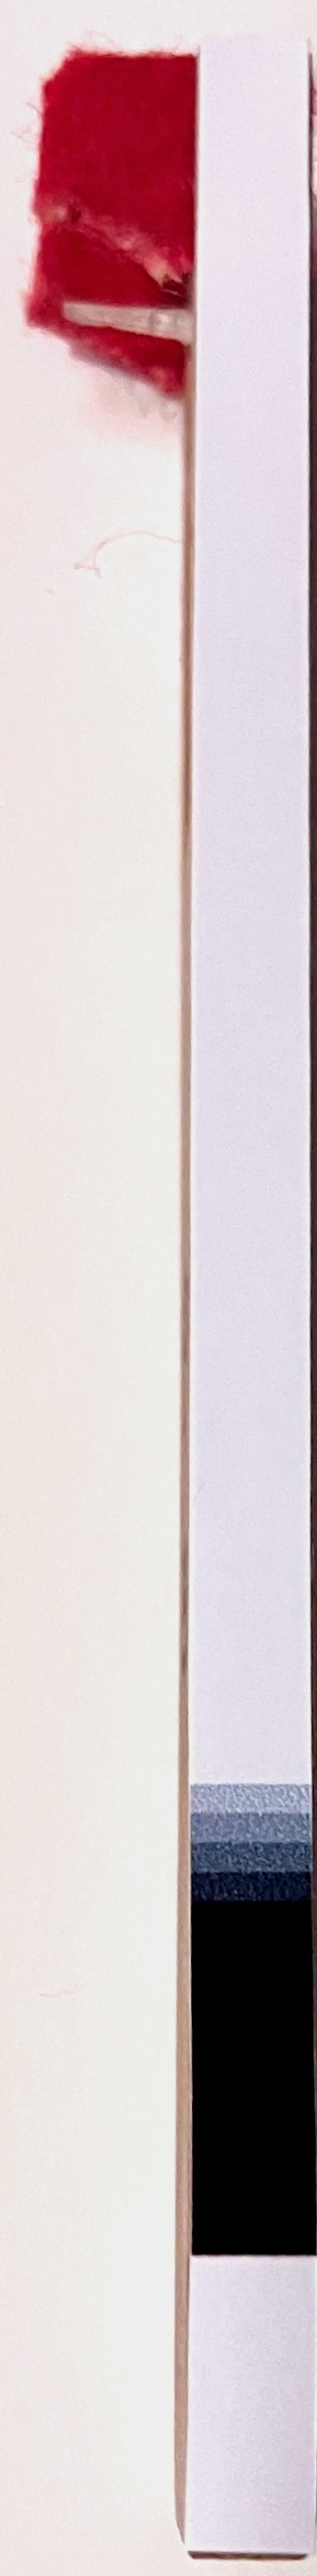
\includegraphics[width=1\linewidth]{img/jack-w-tag.jpeg}
\caption{(Top): Snapshots of the plectrum-string interaction during a pluck. Note how the plectrum initially pushes the string but is eventually pushed back by the string before release. (Bottom): side view of a jack showcasing the colour gradient in the reflecting sticker used by the optical sensing mechanism.}\label{fig:frames}
\end{figure}

\begin{figure}
    \centering
    \includegraphics[width=0.76\linewidth]{img/BOTHvertical.png}
    \caption{
    (a) FSR and optical sensor data for both registers of a key, as recorded by the ADC. 
    \textbf{Th1} and \textbf{Th2} lines are the thresholds for the first and second set of optical sensors.     
    (b) FSR data at 8~kHz sample rate. Black lines show the pluck point for each register. Time difference between plucks: 14~ms (110 samples).    }
    \label{fig:fsr-dif}
\end{figure}


In the current design, FSR signals complement optical data by indicating actual force application. FSRs were installed beneath each jack to detect actual string excitation. Connected in a voltage divider circuit (Figure~\ref{fig:fsr_circuit}), the output voltage reads:
\begin{equation}\label{eq:fsr_circuit}
V_{OUT} = \frac{R_0}{R_0 + R_{FSR}}V_{CC},
\end{equation}
from which the varying sensor's resistance $R_{FSR}$ can be estimated. Such varying resistance can ultimately be converted to a force signal measured in Newton's via a conversion table from the supplier. 

In addition to measuring force magnitudes, the FSR signal functions as a validation layer. When the optical sensor reading exceeds the pluck threshold, the system verifies whether a corresponding rate of change is present in the FSR signal. If no such drop is detected—indicating an absence of string contact—the event is disregarded. As a result, only deliberate plucking gestures lead to sound output, while unintended movements are effectively disregarded. Figure~\ref{fig:fsr-dif}(a) displays the four signals captured from a single key gesture—two per register, representing the optical and force-sensitive sensors. It can be observed that one string is correctly identified as plucked, evidenced by a sharp drop in the force signal (black solid curve), while the second string (red curves), despite the optical threshold being crossed, is not plucked.

Figure~\ref{fig:fsr-dif}(b) shows a time series from both sensors on a single key, sampled at 8~kHz and converted to Newtons. The onset of key motion is marked by displacement without resistance, followed by a sharp drop in the FSR signal that corresponds to the pluck. Together, the optical and force signals show strong temporal alignment across gestures. Based on recordings and sensor data, the delay between register plucks during normal performance ranged from 12ms to 30ms. 


The current configuration supports per-register velocity assignment at note onset, with \texttt{Note\_ON} velocities derived from the peak force measured by the FSR prior to its decay. Since FSRs are insensitive to key release, \texttt{Note\_OFF} velocity is instead estimated from the rate of downward motion, as captured by the optical sensor when crossing the release threshold.



\section{Physical Models and Implementation}

The control interface drives a nonlinear, two-register string model emulating the physical response of early Italian harpsichords. These instruments typically employed yellow brass strings, which, being relatively soft and unable to withstand high tension, contributed—together with the flexible soundboard and thin case sides—to a characteristically bright and sustained tone. For a digital reconstruction to sound convincing, it must account for behaviours like pitch glides, modal coupling, and amplitude modulation. Such features lie beyond the reach of linear string models and require the inclusion of geometric nonlinearities. Consider the following nonlinear model:
\begin{equation}\label{eq:CntModel}
\rho A \partial_t^2 u(x,t) = \mathcal L u(x,t) + \partial_x\phi^\prime_{nl}(\partial_x u) + \delta^{(x_f)}f(t),
\end{equation}
where $u(x,t)$ denotes the transverse displacement; $\rho$ is the material density; $A = \pi r^2$ is the cross-sectional area of a circular string; $\delta^{(x_f)} = \delta(x - x_f)$ is a Dirac delta representing the point of external excitation. The notation $\partial_z^n$ denotes the $n^{\text{th}}$ partial derivative along $z$, and primes ($^\prime$) denote total differentiation. 
The operator $\mathcal L$ models linear dynamics:
\begin{equation}
\mathcal L := T_0 \partial_x^2 - EI \partial_x^4,
\end{equation}
with $T_0$ the string tension, $E$ Young’s modulus, and $I = \pi r^4/4$ the area moment of inertia. The nonlinear potential function $\phi_{nl}$ governs the geometric nonlinearity:
\begin{equation}\label{eq:phiNL}
\phi_{nl}(\partial_x u) := \frac{EA - T_0}{8} (\partial_x u)^4.
\end{equation}
This expression approximates a low-order expansion of the geometrically exact string model (for the full model and a discretisation employing finite elements, see \cite{chabassier2010energy}), sufficient to produce perceptually relevant nonlinear effects such as pitch glides and modal coupling \cite{russo2024scalar}. Note that the interactions with the soundboard and the radiation into the surrounding medium, whilst important for sound synthesis, are neglected at this stage, as they do not influence the structure of the control data stream of this proof-of-concept.

Boundary conditions are taken as simply supported: $u = \partial_x^2 u = 0$ at $x = \{0, L\}$. Applying modal decomposition:
\begin{equation}\label{eq:ModalSystem}
u(x,t) := \sum_{m=1}^M X_m(x) q_m(t) = {\bf X}^\intercal(x) \, {\bf q}(t),
\end{equation}
with $X_m := \sqrt{2/L} \sin\left(\frac{m\pi x}{L}\right)$ and ${\bf q}(t)$ the vector of modal coordinates, results in the following projected system:
\begin{equation}
\ddot {\bf q} = -{\bf \Omega}^2{\bf q} - {\bf C}\dot{\bf q} - \int_{\mathcal I} {\bf X}' \phi^\prime_{nl}\,\mathrm dx + {\boldsymbol \eta} f(t),
\end{equation}
where ${\bf \Omega} := \text{diag}[\Omega_1,...,\Omega_M]$ is a diagonal matrix of eigenfrequencies defined as:
\begin{equation}
\Omega_m = \sqrt{\frac{T_0}{\rho A} \left(\frac{m\pi}{L}\right)^2 + \frac{EI}{\rho A} \left(\frac{m\pi}{L}\right)^4}.
\end{equation}
The diagonal damping matrix ${\bf C} := \text{diag}[2\sigma_1,...,2\sigma_M]$ was arbitrarily added after modal projection, and it approximates the light, uncoupled modal losses. The damping coefficients $\sigma_m$ can be estimated experimentally or be derived from a model such as Cuesta and Vallette's \cite{cuesta1996nonlinear}.

\subsection{Energy quadratisation and time stepping scheme}
The modal system is passive and satisfies the energy balance:
\begin{equation}
\frac{\mathrm d H}{\mathrm dt} = -\dot {\bf q}^{\intercal}{\bf C}\dot{\bf q} + \dot{\bf q}^{\intercal}{\boldsymbol \eta} f(t),
\end{equation}
with total energy:
\begin{equation}
H = \frac{1}{2} \dot{\bf q}^{\intercal} \dot{\bf q} + \frac{1}{2} {\bf q}^{\intercal} {\bf \Omega}^2 {\bf q} + \int_{\mathcal I} \phi_{nl}\,\mathrm dx,
\end{equation}
and note that the energy is strictly decreasing when the source is inactive ($f(t) = 0$). To ensure numerical stability in the presence of nonlinear terms, the system is reformulated using the Scalar Auxiliary Variable (SAV) method \cite{bilbao2023explicit, vanWalstijn_JSV_2024}:
\begin{equation}
\psi := \sqrt{2 \int_{\mathcal I} \phi_{nl}\,\mathrm dx},
\end{equation}
yielding:
\begin{subequations}\label{eq:SAVCnt}
\begin{align}
   \ddot {\bf q} &= -{\bf \Omega}^2{\bf q} - {\bf C}\dot{\bf q} - \psi \nabla_{\bf q}\psi + {\boldsymbol \eta} f(t), \\
   \dot \psi &=  (\nabla_{\bf q}\psi)^\intercal \dot {\bf q}.
\end{align}
\end{subequations}
System~\eqref{eq:SAVCnt} is discretised using staggered time series for ${\bf q}$ and $\psi$. Let ${\bf q}^n \approx {\bf q}(Tn)$ and $\psi^{n-\tfrac{1}{2}} \approx \psi(T(n - \tfrac{1}{2}))$ at time step $n$ and with sampling period $T$. Discrete-time operators are defined as:
\begin{subequations}
\begin{align}
\delta_{2} {\bf q}^n &:= \frac{{\bf q}^{n+1} - 2{\bf q}^n + {\bf q}^{n-1}}{T^2}, \\
\mu_{2} {\bf q}^n &:= \frac{{\bf q}^{n+1} + 2{\bf q}^n + {\bf q}^{n-1}}{4}, \\
\delta_{\cdot} {\bf q}^n &:= \frac{{\bf q}^{n+1} - {\bf q}^{n-1}}{2T}, \\
\delta_{+} \psi^{n-\tfrac{1}{2}} &:= \frac{\psi^{n+\tfrac{1}{2}} - \psi^{n-\tfrac{1}{2}}}{T}, \\
\mu_{+} \psi^{n-\tfrac{1}{2}} &:= \frac{\psi^{n+\tfrac{1}{2}} + \psi^{n-\tfrac{1}{2}}}{2}.
\end{align}
\end{subequations}
Using these, the time-stepping scheme employed here is:
\begin{align*}
   \delta_2 {\bf q}^n &= -\tilde{\bf \Omega}^2 \mu_2{\bf q}^n - \tilde{\bf C} \delta_\cdot {\bf q}^n - \mu_{+}\psi^{n-\tfrac{1}{2}} {\bf g}^n + {\boldsymbol \eta} f^n, \\
   \delta_{+} \psi^{n-\tfrac{1}{2}} &= ({\bf g}^n)^\intercal \delta_{\cdot} {\bf q}^n, \\
   {\bf g}^n &:= (\nabla_{\bf q} \psi)\big|_{t = Tn},
\end{align*}
where:
\begin{align*}
\tilde \Omega^2_m &:= \frac{4}{T^2}\frac{1-2e^{-\sigma_m T}\cos(T\sqrt{\Omega_m^2-\sigma_m^2})+e^{-2\sigma_m T}}{1+2e^{-\sigma_m T}\cos(T\sqrt{\Omega_m^2-\sigma_m^2})+e^{-2\sigma_m T}}, \\
\tilde \sigma_m &:= \frac{2}{T}\frac{1-e^{-\sigma_m T}}{1+2e^{-\sigma_m T}\cos(T\sqrt{\Omega^2_m-\sigma_m^2})+e^{-2\sigma_m T}}.
\end{align*}
This discretisation has several desirable properties. First, it ensures that the linear part is discretised exactly \cite{cieslinski2011exact}, as it appears in previous works employing modal synthesis \cite{vanWalstijn_DAFX_2016,vanWalstijn_JSV_2024}. Second, it is unconditionally stable. Finally, the system's update -not shown here for brevity- is performed explicitly via the Sherman-Morrison formula \cite{bilbao2023explicit,russo2024scalar,shermanAMS1950}, avoiding nonlinear root finding algorithms -often requiring several iterations per time step- or large matrix inversions.

To manage computational complexity further, full nonlinearity is applied only to modes below 3\,kHz; higher modes are treated linearly. This hybrid approach preserves perceptual features while reducing floating-point cost. Additionally, a constrained version of the SAV method, adapted from \cite{vanWalstijn_JSV_2024}, is employed to enforce the non-negativity of $ \mu_{t+}\psi^{n-\frac{1}{2}}$, preventing spurious numerical artefacts from appearing in the solution and allowing the auxiliary variable to decay toward zero. %A slightly altered formulation is employed, as presented by Russo \emph{et al.}~ 
A detailed description can be found in \cite{russo2024guitar, russo2025phd}.






% ---------------------------------------------------------------------------------
% CJW section START

\section{Real-Time Software Implementation}

The software component of the prototype system consists of a real-time instrument plug-in (VST3/Audio Unit), designed for integration with standard Digital Audio Workstations (DAWs). The selected DAW must support the transmission of MIDI channel information to the active track, enabling multi-channel polyphonic expression (MPE)-style communication.

\subsection{System Overview}

The software simulates a pair of nonlinear strings, forming a single voice whose pitch is determined by the mechanically actuated key. For the purposes of computational benchmarking, low-pitched notes were selected: specifically, C2 (65\,Hz), along with the adjacent C\#2 and D2. Each string is modelled with a length of 2\,m and a radius of 0.3\,mm, employing appropriate material parameters for brass.

The system processes \texttt{Note\_ON} and \texttt{Note\_OFF} events received over two independent MIDI channels, supporting individual excitation and damping of each string and preserving temporal offsets between the associated jacks. These MIDI events may span multiple processing buffers; therefore, each is timestamped and rendered within the correct frame. Additional components include an excitation signal and jack noise, as illustrated in Figure~\ref{fig:software diagram}.

\begin{figure}
    \centering
    \includegraphics[width=7cm]{img/SoftwareDiagram.pdf}
    \caption{Real-time system implementation comprising a pair of nonlinear strings triggered by MIDI signals distributed across multiple buffers.}
    \label{fig:software diagram}
\end{figure}

Excitation is applied as a time-limited forcing term at a designated point along each string, informed by the pressure sensor beneath the mechanical key. The excitation signal, approximately 50\,ms in duration, is selected via linear interpolation between two stored waveforms, based on the MIDI \texttt{Note\_ON} velocity. Additionally, the sound of the jack returning to its rest position is incorporated via a pre-recorded noise sample. The \texttt{Note\_OFF} velocity is used to modulate the amplitude of this signal prior to mixing with the output audio.

\subsection{Computational Challenges}

The use of nonlinear modal string synthesis in a real-time audio environment is computationally demanding, both at the model initialisation phase (\texttt{Note\_ON}) and during continuous audio rendering at each time step. In contrast to a linear string model—which requires a single vector update and dot product per time step—the nonlinear system entails substantially more operations. For instance, the C2 note requires a modal resolution of 150 modes. Each time step involves two matrix-vector multiplications, seven vector updates, and six dot products. When matrices are square, multiplication accounts for over 80\% of the total computational load.

To attain viable single-core CPU performance, both algorithmic and low-level code optimisations were implemented. As mentioned previously, one effective strategy involved partitioning the modal range into two segments: a low-to-mid frequency band up to approximately 3\,kHz, and a higher frequency band extending to the upper modal limit. The lower segment (approximately 50 modes for C2) is computed using the full nonlinear model, whereas the higher modes are updated using a simplified linear routine. This segmentation reduces matrix dimensionality and lowers the cost of associated vector operations. With this approach, CPU usage per string was reduced to approximately 10\%. Further optimisation is anticipated through under-sampling of the nonlinear modal segment.

Beyond real-time rendering, the initialisation of each string model introduces additional processing overhead. Specifically, the computation of modal shapes—involving thousands of trigonometric evaluations at each \texttt{Note\_ON} event—can lead to transient CPU load spikes, potentially causing buffer under-runs. To mitigate this, a caching system for precomputed modal matrices is recommended for scalable polyphonic implementation.


% CJW section END
% ---------------------------------------------------------------------------------



\section{Discussion and Conclusion}

The system presented in this paper builds upon previous work on sensor-augmented harpsichord interfaces—most notably the San Colombano project \cite{hamilton2025augmentation}—by introducing substantial refinements in both gesture detection and synthesis integration. While earlier designs relied solely on optical displacement tracking, the present system introduces a dual-sensor architecture, combining reflective optical sensors with force-sensitive resistors (FSRs). This hybrid approach enables robust pluck detection through velocity-sensitive hysteresis and force validation, reducing false positives, particularly during complex or expressive gestural input. These developments address known shortcomings of threshold-based detection and allow for a more reliable mapping between mechanical gestures and sonic outcomes. The current prototype setup is visible in Figure \ref{fig:setup}. 



\begin{figure}
    \centering
    \includegraphics[width=\linewidth]{img/project-setup-3.jpeg}
    \caption{The prototype setup, showing the three-key harpsichord model connected to a 2023 MacBook Pro. The prototype VST is visible, along with a list of triggered MIDI messages.}
    \label{fig:setup}
\end{figure}



Conventional digital control of plucked keyboard instruments suffers from several shortcomings, namely: the lack of control resolution in standard MIDI devices, the inability to articulate register-specific timing offsets, and the absence of mechanical feedback needed for historically informed performance. The proposed system addresses these challenges through a custom-built harpsichord mechanism with staggered dual-register jacks, paired with real-time gesture tracking and nonlinear physical modelling. The resulting interface supports temporally resolved articulation across registers, required for expressive control.

From the perspective of sound synthesis, the system incorporates a physically realistic, nonlinear string model that supports two independently plucked registers per key. By constraining nonlinear computations to low-order modes (below 3\,kHz), and employing a modal energy quadratisation scheme with a constrained Scalar Auxiliary Variable (SAV), the model achieves a balance between physical fidelity and computational tractability. As a result, real-time synthesis is attained on consumer-grade hardware with a CPU footprint of approximately 10\% per voice on the most computationally demanding strings in the bass register, while preserving key nonlinear characteristics such as pitch glides and modal coupling.

The prototype shows that a high level of expressivity can be achieved through targeted hardware augmentation and physics-informed synthesis. It reaffirms the value of context-specific interfaces when coupled with physically grounded models, particularly in the domain of historically informed digital instrument design. Future work will extend the current architecture to a full keyboard, explore enhanced mapping strategies for velocity and dynamics, and incorporate more detailed models of soundboard interaction and acoustic radiation.


